% author: xiaoyaowudi

\documentclass[UTF8]{ctexart}
\usepackage{amsmath}
\usepackage{minted}
\usepackage{amssymb}
\usepackage{graphicx}
\usepackage{float}
\usepackage{url}
\CTEXsetup[format={\bfseries}]{section}
\title{乒乓球发球机制作报告}
\author{黑暗森林小组: 肖子尧, 杨烨泽, 陆中天}
\date{\today} 
\usepackage[a4paper,left=10mm,right=10mm,top=15mm,bottom=15mm]{geometry}
\begin{document}
\vspace*{\fill}
\begin{center}
      {\Huge 乒乓球发球机制作报告}\\[0.5cm]
      {\Large 黑暗森林小组: 肖子尧, 杨烨泽, 陆中天}\\[0.4cm]
      {\today}\\[0.4cm]
      {消灭人类暴政, 世界属于我们!}
\end{center}
\vspace*{\fill}
\newpage
\tableofcontents
\newpage
\section{\Large 简介}
考虑到目前大多数简易乒乓球发球机无法回收利用乒乓球, 我们小组决定制作一个可以回收再利用乒乓球的乒乓球发球机. 并且可以调整距离远近与发球频率, 打出上旋球和下旋球, 还可以更换供球方式. 下图为成品侧视图
\begin{figure}[H]
\centering
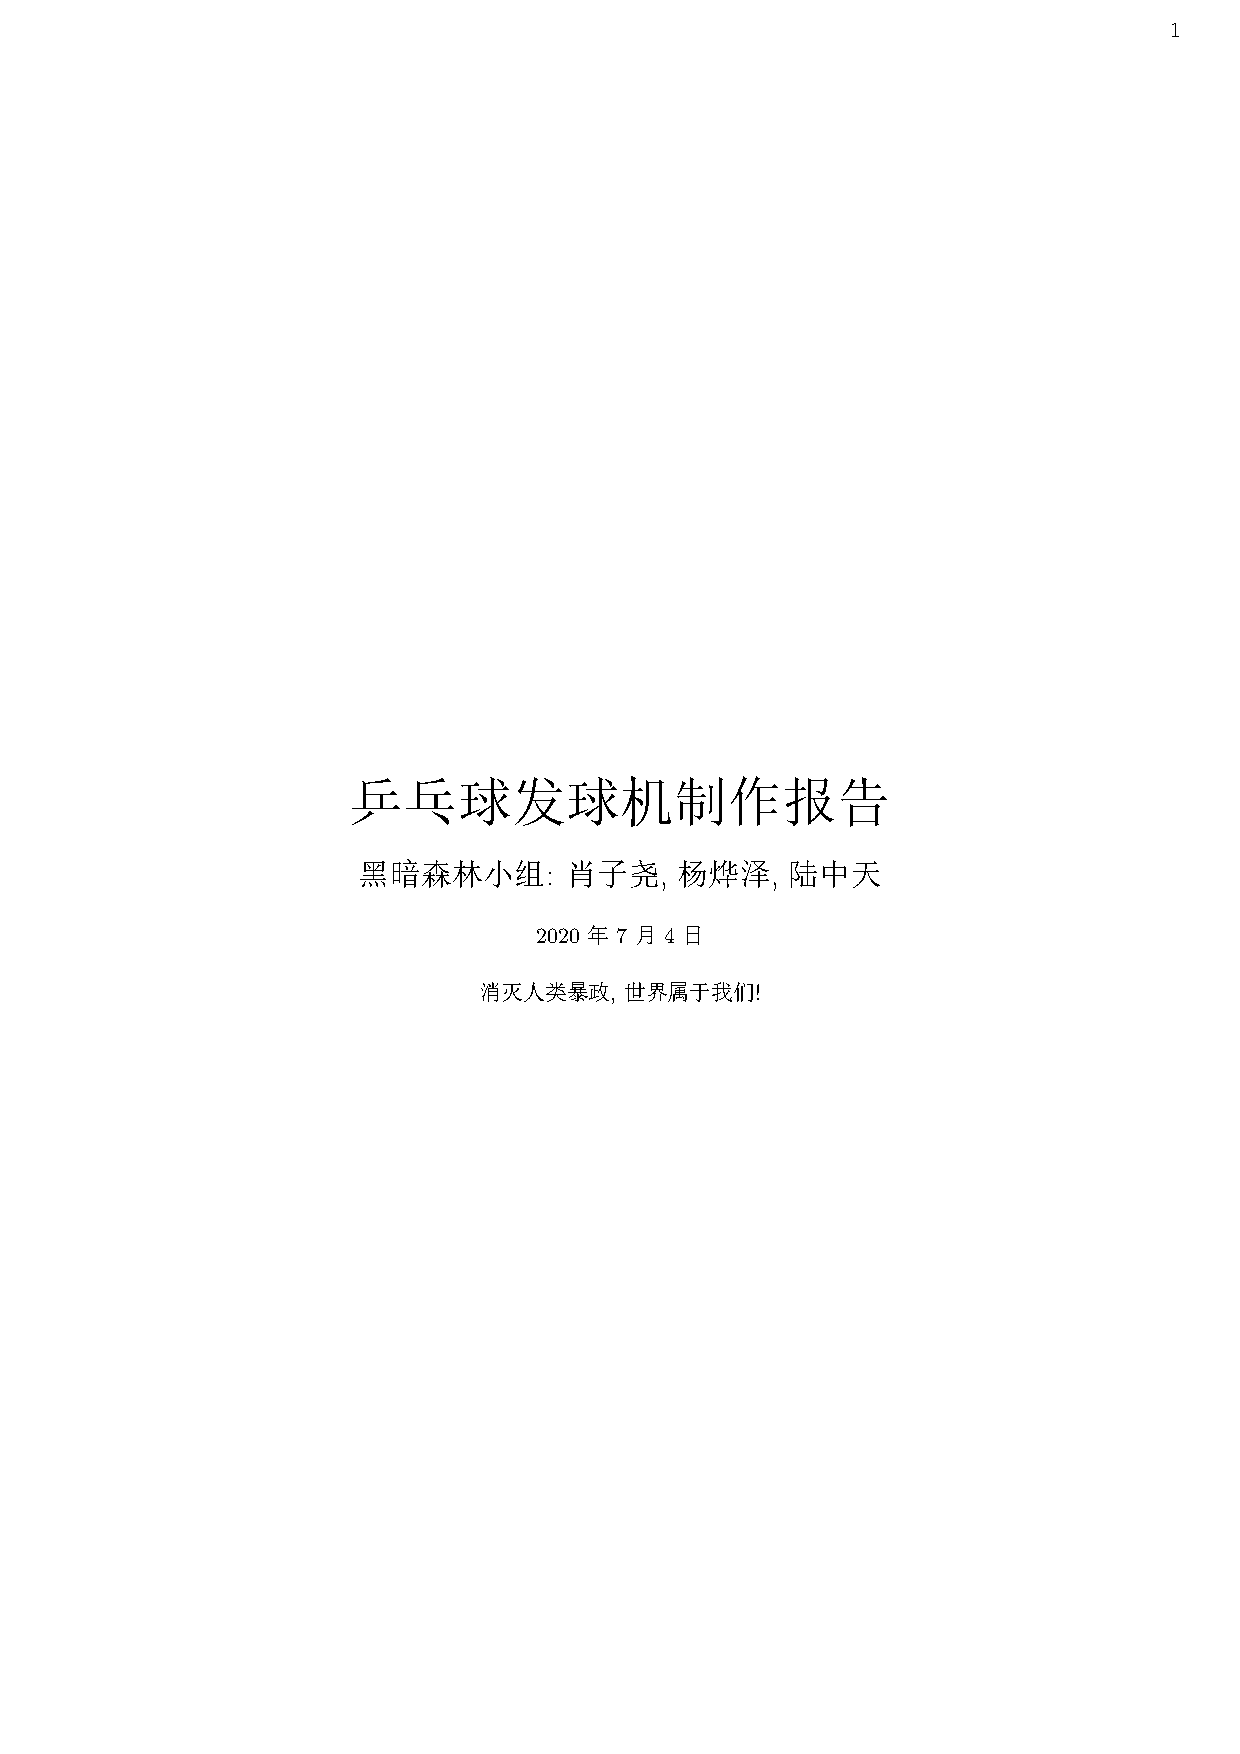
\includegraphics[width=0.80\textwidth, angle=270]{machine.jpg}
\caption{成品侧视图}
\end{figure}
\section{\Large 结构}
这个发球机主体结构主要分为四个部分:供球导轨部分, 供球动力部分, 发球部分, 支架部分.
\subsection{\large 供球导轨部分}
供球导轨采用了正方形接口, 既可以装配网袋回收利用球, 也可以直接使用箱子等容器供球. 导轨部分主要功能为将球一个一个排列好送入供球动力部分, 下图为该部分侧视图.
\begin{figure}[H]
\centering
\includegraphics[width=0.13\textwidth]{rail.jpg}
\caption{供球导轨部分侧视图}
\end{figure}
\subsection{\large 供球动力部分}
供球动力部分使用履带方式将球从导轨运至上半部分, 并用下层的球推动的上层的球进入发球部分. 下图为该部分侧视图.
\begin{figure}[H]
\centering
\includegraphics[width=0.12\textwidth]{sport.jpg}
\caption{供球动力部分侧视图}
\end{figure}
\subsection{\large 发球部分}
发球部分使用两个可独立调速的高速电机发球, 下图为该部分侧视图.
\begin{figure}[H]
\centering
\includegraphics[width=0.12\textwidth]{eject.jpg}
\caption{发球部分侧视图}
\end{figure}
\subsection{\large 支架部分}
支架部分使用两块木板以及两个三角结构支撑整个发球机, 下图为该部分侧视图.
\begin{figure}[H]
\centering
\includegraphics[width=0.12\textwidth]{support.jpg}
\caption{支架部分侧视图}
\end{figure}
\section{\Large 功能}
此发球机可以实现供球方式和发球的多样性.
\subsection{\large 多样化供球方式}
由于本发球机的乒乓球导轨入口低于桌面, 因此可以使用网袋回收训练者击打回的乒乓球.此外, 可以很方便的更换供球方式, 只需将储存乒乓球的容器接在导轨口或将网袋系在导轨口即可.此功能提供便捷的回收方式, 并且能很快的适应不同的使用场景.此功能解决了大部分轻便型发球机只能使用垂直供球方式导致无法回收球的缺点, 并且也可以使用垂直供球.
\subsection{\large 发球}
此发球机的两个摩擦轮由两个独立的调速电控控制, 并且旋转轴平行于桌面, 因此本发球机可以实现方便地控制发球的落点, 以及发出的乒乓球的上下旋.此功能解决了一些轻便型发球机使用的旋转轴垂直于桌面导致无法上下旋的缺点.
\section{\Large 优缺点及创新性分析}
\noindent 本发球机经过测试, 具有以下几个优缺点及创新点\\
\large{优点}:
\begin{itemize}
	\item 实现垂直供球及网袋回收利用两种供球方式
	\item 可以方便控制发球初速以及发球旋转方式
	\item 最复杂的供球部分使用可方便替换的 \textit{\textbf{LEGO}} $ ^\text{TM} $ 零件 \footnote{一种积木玩具}, 稳定性强, 方便维修
	\item 整个装置非常轻便, 质量远小于同类发球机
	\item 此发球机具有完全自主知识产权
	\item 此发球机制作成本极低
	\item 安装步骤较为简单
\end{itemize}
\large{缺点}:
\begin{itemize}
	\item 供球部分总长度较长, 需要较多的乒乓球
	\item 无法控制水平发球方向, 无法实现球的左右旋
	\item 此发球机并未使用任何形式的存储器, 无法记忆发球参数
	\item 此发球机整体使用木头, PVC塑料, ABS塑料等材质, 强度较低
\end{itemize}
\large{创新点}:
\begin{itemize}
	\item 采用模块化接口, 可更换供球方式
	\item 在发球机上采用 \textit{\textbf{LEGO}} $ ^\text{TM} $ 零件, 节省制作复杂度, 并可以方便的更换减速模块改变发球频率
	\item 使用履带供球,更稳定高效
\end{itemize}
\section{\Large 后期改进方向}
\noindent 基于上述缺点, 我们确定了一下几个后期改进方向:
\begin{itemize}
	\item 使用Raspberry Zero \footnote {基于Linux的小型低价单片机电脑} 控制电机, 可以方便地储存并应用各种发球参数
	\item 使用减速电机制作活塞, 驱动发射部分来回摆动做到调整控制水平方向
	\item 做到发射部分可旋转使得发射的球可以任意角度旋转
\end{itemize}
\section{\Large 各部分技术选择及原因}
我们首先同时制作发球部分与供球动力部分, 然后制作了支架部分, 最后制作了供球导轨部分.
\subsection{\large 发球部分}
乒乓球直径为40mm \footnote{国际乒联自2014年7月1日起规定国际乒乓球标准直径为40.00mm至40.60mm} , 因此我们将两个高速电机带动的摩擦轮之间的距离定为39.00mm \footnote{误差 $ \pm $ 0.5mm}, 提供的木板并没有合适的对称螺孔安装电机, 并且若将电机安装至给定的木板上, 摩擦轮的垂直直径较小导致两个摩擦轮无法固定乒乓球的任意一条直径, 发射的球方向不确定, 因此我们决定在木板上钻孔安放电机, 并使用PVC管制作供球部分到发球部分的导轨以及发球部分左右两块木板之间长度为 4.3mm \footnote{误差 $ \pm $ 1mm} 的支架. 此后我们将电池与电机电控置于发球部分侧面使得其易于控制, 但缺点是无记忆芯片, 无法记录发球参数.
\subsection{\large 供球动力部分}
若使用提供的减速电机制作的叶片将乒乓球从低处运到高处, 叶片的制作以及乒乓球的导轨的制作将变得极其复杂. 因此我们首先考虑使用减速电机搭配摩擦轮将乒乓球从低处运至高处, 但这样将导致我们必须使用软管, 装置强度过低, 无法固定. 我们考虑使用 \textit{\textbf{LEGO}} $ ^\text{TM} $ 零件, 使用履带加上固定装置, 以及由齿轮制作的减速装置来将乒乓球从低处运至高处, 并推动上层导轨的乒乓球, 将其运送至发球部分. 这样做使得装置稳定性好, 模块化, 易于更换, 质量远小于同类零件, 易于固定, 缺点是强度略低于钢质结构.
\subsection{\large 支架}
由于发球部分的质量在各部分中质量占比最大, 并且供球动力部分与发球部分之间采用热熔胶连接, 强度较低, 因此我们使用PVC管制作了两个三角支架, 并连接到底部的两块支撑木板, 使得整个发球机的重心位于支撑木板上, 不会倾倒.
\subsection{\large 供球导轨部分}
若在此部分使用软管将乒乓球一一排列送入供球动力部分, 软管无法较好地与供球动力部分的 \textit{\textbf{LEGO}} $ ^\text{TM} $ 零件连接, 可能出现连接不稳定, 卡球等情况, 并且不易于固定. 因此我们在这一部分也使用 \textit{\textbf{LEGO}} $ ^\text{TM} $ 零件, 可以方便地将球一一分离并送入供球动力部分的履带. 这里我们使用了正方形的接口, 既可以方便地接其他 \textit{\textbf{LEGO}} $ ^\text{TM} $ 零件, 很好地被其他部分固定, 也可以方便地固定网袋或其他乒乓球储存容器的圆形接口, 简化乒乓球输入.
\section{\Large 结束语}
我们的发球机兼顾了实用性, 简便性, 美观性, 创新性. 创新地应用了一部分技术, 且功能齐全, 较为美观. 但仍有一些缺点仍需改进.
\section{\Large 鸣谢}
\noindent 特别鸣谢: 叶蔚然, 王晓轩, 万鹤荣 \\
\noindent 参考文献:
\begin{itemize}
	\item[ [1] ] \url{https://zh.wikipedia.org/wiki/%E4%B9%92%E4%B9%93%E7%90%83}
	\item[ [2] ] \url{https://zh.wikipedia.org/wiki/%E6%A0%91%E8%8E%93%E6%B4%BE}
	\item[ [3] ] \url{https://zh.wikipedia.org/wiki/%E6%A8%82%E9%AB%98}
\end{itemize}
\section{\Large 附录}
\begin{itemize}
	\item[ [1] ] 论文源码文件及图片文件: \url{https://github.com/xiaoyaowudi-extreme/machine}
\end{itemize}
\begin{figure}[H]
\centering
\includegraphics[width=0.80\textwidth]{blackhole.jpg}
\end{figure}
\end{document}